\begin{tikzpicture}[scale=\trackingExampleScale, every node/.style={transform shape}]
    \begin{scope}[baseline=(image1.south)]
        \node (image1) {
            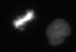
\includegraphics[width=0.25\textwidth]{images/cell_tracking/example_00.png}
        };
        \node[transparent_node, red, xshift=-12pt, yshift=5pt] (d11) at (image1.center) {}; 
        \node[transparent_node, green, xshift=20pt, yshift=-5pt] (d12) at (image1.center) {}; 
    \end{scope}
    \begin{scope}[baseline=(image2.south)]
        \node[right=of image1, xshift=-20pt] (image2) {
            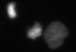
\includegraphics[width=0.25\textwidth]{images/cell_tracking/example_01.png}
        };
        \begin{scope}[overlay]
            \node[transparent_node, red, xshift=-25pt, yshift=15pt] (d21) at (image2.center) {}; 
            \node[transparent_node, green, xshift=18pt, yshift=-10pt] (d23) at (image2.center) {};
            \path[assignment_arrow, red, bend left=20] (d11) edge (d21);
            \path[assignment_arrow, green, bend right=20] (d12) edge (d23.south west);
        \end{scope}
    \end{scope}
    \begin{scope}[baseline=(image3.south)]
        \node[right=of image2, xshift=-20pt] (image3) {
            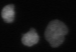
\includegraphics[width=0.25\textwidth]{images/cell_tracking/example_02.png}
        };
        \begin{scope}[overlay]
            \node[transparent_node, red, xshift=-26pt, yshift=13pt] (d31) at (image3.center) {}; 
            \node[transparent_node, green, xshift=18pt, yshift=-8pt] (d33) at (image3.center) {}; 
            \path[assignment_arrow, red, bend left=20] (d21) edge (d31);
            \path[assignment_arrow, green, bend right=35] (d23.south east) edge (d33.south west);
        \end{scope}
    \end{scope}
\end{tikzpicture}


%%% Local Variables: 
%%% mode: latex
%%% TeX-master: "../../../main"
%%% End: 
